\documentclass[../main.tex]{subfiles}
\begin{document}

\chapter{Lecture 13 - 27-04-2020}

\section{Linear prediction}

We had $ERM$ $\hat{h}$
\\
$$
S = \{(x_1,y_1) ... (x_n,y_n) \} \qquad x_t \in \barra{R}^d \qquad y_t \in \{-1,+1\} \qquad \ell_t(w) = I \{ y_t w^T x_t \leq 0 \}
$$

$$
\hat{h}_S = arg \min_{h\in H_D} \frac{1}{m} \sum_{t = 1}^{m} I \{ y_t w^T x_t\} \leq 0 
$$
The associated decisio problem is a NP problem so cannot be camputed efficientiy unless $P \equiv NP$
\\
Maybe we can approximate it, so a good solution that goes close to minimise error.
\\
This is called MinDisOpt\\

\subsection{MinDisOpt}
Instance: $(x_1,y_1) ...(x_n, y_n) \in \{0, 1 \}^d x\{0,1\}$

Solutio: 
$$w \in Q^D \textbf{minimising the number of indices} t = 1,...m \ s.t. \
h_t w^Tx_t \leq 0 
$$
$Opt(S)$ is the smallest number of mislcassified example in S by any linear classifier in $H_D$ 
\\
where $\frac{Opt(S)}{m}$ is training error of $ERM$
\\\\
\bred{Theorem} : if $P \not \equiv NP$, then $\forall c > 0$ there are no polytime algorithms (with r. t. the input size $ \Theta(m_d)$) that approximately solve every istance $S$ of MinDisOpt with a number of mistakes bounded by $C \cdot Opt(S)$.\\
If I am able to approximate it correclty this approximation will grow with the size of the dataset.
\\\\
$$\forall A \ \textbf{(polytime)} \ \ and \ \ \forall C \quad \exists S \qquad \hat{\ell}_S\left(A\left(S\right)\right) \geq c \cdot \hat{\ell}_S\left( \hat{h}_S \right) \ \textbf{(where $\hat{h}_S$  is $ERM$)}
$$

$$
Opt(S) = \hat{\ell}_S(\hat{h}_S)
$$
\\
This is not related with free lunch theorem (information we need to get base error for some learning problem). Free lunch: we need arbitrarirally information to get such error.
Here is we need a lot of computation to approximate the $ERM$. 
\\\\
Assume $Opt(S) = 0 $ $ERM$ has zero training error on $S$\\
$\exists U \in \barra{R}^d$ \ s.t. \ $\forall t = 1 , ...m$ \qquad $y_tU^Tx_t > 0$ \qquad \bred{$S$ is linearly separable}\\
\begin{figure}[h]
    \centering
    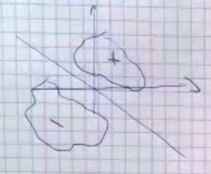
\includegraphics[width=0.6\linewidth]{../img/lez13-img1.JPG}
    \caption{Tree building}
    %\label{fig:}
\end{figure}
\\
We can look at the min
$$
\min_{t=1,...m} y_t U^T x_t = \gamma(U) > 0 \qquad \bred{We called this marginn of $U$ on $(x_t,y_t)$}
$$ 
\\
We called in this way since $\frac{\gamma(U)}{\| U \|} = \min{t} y_t \| x_t\| cos(\Theta)
$
\begin{figure}[h]
    \centering
    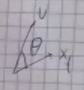
\includegraphics[width=0.2\linewidth]{../img/lez13-img2.JPG}
    \caption{Tree building}
    %\label{fig:}
\end{figure}\\
\\
where $\Theta$ is the angle
\\
\begin{figure}[h]
    \centering
    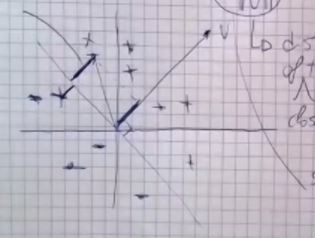
\includegraphics[width=0.6\linewidth]{../img/lez13-img3.JPG}
    \caption{Tree building}
    %\label{fig:}
\end{figure}\\
$where \frac{\gamma(U)}{\|U\|}$ is the distance separating hyperplane on closest training example .
\\\\
S linearly separable and if i look at the sistem of this linear inequality:
$$
\begin{cases}
y_t w_T x_t > 0 \\
y_m w_T x_m > 0 \\
\end{cases}
$$
We can solve it in polytime using a linear solver. So any package of linear programming, and will be solved in linear time.
\\\\
This is called \bred{feasibilty problem}. We want a point $y$ that satisfy all my linear inequalities.
\\
\begin{figure}[h]
    \centering
    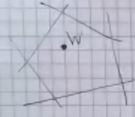
\includegraphics[width=0.2\linewidth]{../img/lez13-img4.JPG}
    \caption{Feasibilty problem}
    %\label{fig:}
\end{figure}\\
\\ 
\textbf{When $Opt(S) = 0 $ is  we can implememtn $ERM$ efficiently using LP (Linear programming).} \\They may overfitting since a lot of bias. When this condition of Opt is no satisfy we cannot do it efficiently. 
LP algorithm can be complicated so we figure out another family of algorithm.

\section{The Perception Algorithm}
This came from late '50s and was designed for psicology but have a general utility in othe fields.
\\\\
Perception Algorithm\\
Input : training set $S = \{ (x_t,y_t) ...(x_m, y_m) \}$ \qquad $x_t \in \barra{R}^d \qquad y_t \in \{-1, +1\}
$
Init: $w = (0,...0)$\\
Repcat\\
\quad read next $(x_t,y_t)$\\
If $y_t w^T x_t \leq$ then $w \longleftarrow w +y_t x_t$\\
Until margin greater than 0 $\gamma(w) > 0$ // w separates $S$\\
Output $w$
\\\\
We know that $\gamma(w) = \min_t y_t w^T x_t \leq 0$
The question is, will it terminate if $S$ is linearly separable?
\\
If $y_t w^T x_t \leq 0$, then $w \longleftarrow w + y_t x_t$\\
\begin{figure}[h]
    \centering
    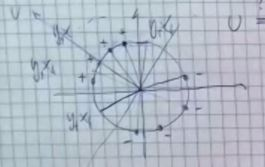
\includegraphics[width=0.3\linewidth]{../img/lez13-img5.JPG}
    \caption{}
    %\label{fig:}
\end{figure}\\
For simplicity our x are in this circle. Some are on the circonference on top left with $+$ sign and some in bottom right with $-$ sign.
\\All minus flipped to the other side and the we can deal the $+$. \\
U is a separating hyperplane, how can i find it?\\
Maybe i can do something like the average: \\$$U = \frac{1}{m} \sum_{t=1}^{m} y_t x_t \ \ ?$$ \\
But actually don't take the average of all of them.
So do not take average of all, instead take the one that satisfy $y_t w^T x_t \leq 0$ condition.
\\
$y_t w^T x_t \leq 0$ is a violated consstraint and we want it $> 0$.
\\
Does $w \longleftarrow w + y_t x_t$ fix it?
$$y_t( w + y_t \cdot x_t)^T x_t = y_t w^T x_t + \| x_t\|^2$$
We are trying to see what happen before and after the updates of w.\\
SInce $\| x_t \| > 0$ so is positive, the update increase margins, thus going towards fixing violated constraints. 
\\\\
\subsection{Perception convergence Theorem}
dated early 60s
On a linearly separable $S$, perceptron will converge after at most $M$ updates (when they touch in the figure) where:
$$
M \leq \left( \min_{U \, : \, \gamma(U) \, =\,1} \| U \|^2 \right)  \left( \max_{t=1,..m} \| x_t\|^2\right)
$$
Algorithm is not able to do that. ALgorithm keeps looking till he get a violating constraint and then stops. This is bounded by the number of loops. 
\\\\
We said that $\gamma(U) = \min_{t} y_t U^T x_t$ > 0 \qquad when $U$ is separator.
\\
$$ \forall t \quad y_t U^T x_t \geq \gamma(U) \quad \Leftrightarrow \quad \forall t \quad y_t \left( \frac{U}{\gamma(U)} \right)^T x_t \geq 1
$$
\begin{figure}[h]
    \centering
    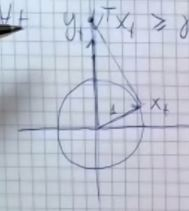
\includegraphics[width=0.3\linewidth]{../img/lez13-img6.JPG}
    \caption{}
    %\label{fig:}
\end{figure}\\
If i rescale U i can make the margin bigger (in particolar $> 1$)\\
The shortest $min \| U \|$ \ s.t. \ $y_t U^T x_t \geq 1$ \quad $\forall t$
\\\\
\bred{Proof}:
\\
$W_m$ is local variable after $M$ updates, I have zero vector \ $W_0 = (0,...0)$
\\
$t_M$ is the index of training example that causes the $M$-$th$ update.\\\\
We want to upper bound $M$ (deriving upper and lower bound \\on a certain quantity $\| W \|$ $\| U\|$)
\\
where $U$ is any s.t. $y_t U^T x_t \geq 1$ \ $\forall t$ 
$$
\| W_M\|^2 = \|W_{M-1} + y_{tM} x_{tM} \|^2 = \|W_{M-1}\|^2 + \|  y_{tM} x_{tM} \|^2 + 2 \cdot y_{tM} W_{M-1}^T x_{tM} \ = 
$$
$$
= \  \|W_{M-1}\|^2 + \| x_{tM}\|^2 + 2 \cdot \red{y_{tM} W^T_{M-1} x_{tM}} \ \leq
$$
where $\red{y_{tM} W^T_{M-1} x_{tM}} \leq 0$
$$
\leq  \ \| w_{M-1}\|^2 + \| x_{tM}\|^2
$$

$$
\| W_M\|^2 \leq \| W_0 \| ^2 + \sum_{i=1}^{M} \|x_t  \|^2 \leq M \ \left( \max_t \| x_t \|^2 \right)
$$
........

.....

...
MANCA  ?????

$$
\| W_M\| \ \|U \| \  \leq \ \| U \| \ \sqrt[]{M} \ \left( \max_t \| x_t \|\right)
$$
since $\cos \Theta \in \left[-1,1\right]$
$$
\|W_M \| \ \| U \| \geq \| W_M \| \ \| U\| \ \cos \Theta = W_M^T U = \left( W_{M-1} + y_{tM} x_{tM} \right)^T U \ = 
$$
where last passage is the \bred{Inner product}
\\
$$
W^T_{M-1} U + \red{y_{tM} U^T x_{tM} } \geq W_{M-1}^T U +1 \geq W_0^T U + M = M
$$
where $\red{y_{tM} U^T x_{tM} }$ is $\geq 1$
$$
M \leq \| W_M \| \ \| U \| \leq \| U \| \ \sqrt[]{M} \left( \max_t \| x_T \| \right)
$$
$$
M \leq \left( \| U\|^2 \right) \left( \max_t \|x_t\|^2 \right) \qquad \forall U \ : \ \min_t y_t U^t x_t \geq 1
$$
$$
M = \left( \min_{U \, : \, \gamma(U) = 1} \| U \|^2 \right) \left( \max_t \| x_t \|^2 \right)
$$\\
Some number depends on $S$
\\
$M$ can be exponential in $md$ when the ball of positive and negative are very closer and the length of $U$ is super long and exponential in $D$.
\\
If dataset barely separable then perceptron will make a number of mistakes that is exponential in the parameter of the problem. 
U is a linear separator and has exponential length
\end{document}
